\documentclass[]{book}
\usepackage{lmodern}
\usepackage{setspace}
\setstretch{2}
\usepackage{amssymb,amsmath}
\usepackage{ifxetex,ifluatex}
\usepackage{fixltx2e} % provides \textsubscript
\ifnum 0\ifxetex 1\fi\ifluatex 1\fi=0 % if pdftex
  \usepackage[T1]{fontenc}
  \usepackage[utf8]{inputenc}
\else % if luatex or xelatex
  \ifxetex
    \usepackage{mathspec}
  \else
    \usepackage{fontspec}
  \fi
  \defaultfontfeatures{Ligatures=TeX,Scale=MatchLowercase}
\fi
% use upquote if available, for straight quotes in verbatim environments
\IfFileExists{upquote.sty}{\usepackage{upquote}}{}
% use microtype if available
\IfFileExists{microtype.sty}{%
\usepackage{microtype}
\UseMicrotypeSet[protrusion]{basicmath} % disable protrusion for tt fonts
}{}
\usepackage[margin=1in]{geometry}
\usepackage{hyperref}
\hypersetup{unicode=true,
            pdftitle={Dissertation Defense},
            pdfauthor={Kirk Gosik},
            pdfborder={0 0 0},
            breaklinks=true}
\urlstyle{same}  % don't use monospace font for urls
\usepackage{natbib}
\bibliographystyle{apalike}
\usepackage{color}
\usepackage{fancyvrb}
\newcommand{\VerbBar}{|}
\newcommand{\VERB}{\Verb[commandchars=\\\{\}]}
\DefineVerbatimEnvironment{Highlighting}{Verbatim}{commandchars=\\\{\}}
% Add ',fontsize=\small' for more characters per line
\usepackage{framed}
\definecolor{shadecolor}{RGB}{248,248,248}
\newenvironment{Shaded}{\begin{snugshade}}{\end{snugshade}}
\newcommand{\KeywordTok}[1]{\textcolor[rgb]{0.13,0.29,0.53}{\textbf{{#1}}}}
\newcommand{\DataTypeTok}[1]{\textcolor[rgb]{0.13,0.29,0.53}{{#1}}}
\newcommand{\DecValTok}[1]{\textcolor[rgb]{0.00,0.00,0.81}{{#1}}}
\newcommand{\BaseNTok}[1]{\textcolor[rgb]{0.00,0.00,0.81}{{#1}}}
\newcommand{\FloatTok}[1]{\textcolor[rgb]{0.00,0.00,0.81}{{#1}}}
\newcommand{\ConstantTok}[1]{\textcolor[rgb]{0.00,0.00,0.00}{{#1}}}
\newcommand{\CharTok}[1]{\textcolor[rgb]{0.31,0.60,0.02}{{#1}}}
\newcommand{\SpecialCharTok}[1]{\textcolor[rgb]{0.00,0.00,0.00}{{#1}}}
\newcommand{\StringTok}[1]{\textcolor[rgb]{0.31,0.60,0.02}{{#1}}}
\newcommand{\VerbatimStringTok}[1]{\textcolor[rgb]{0.31,0.60,0.02}{{#1}}}
\newcommand{\SpecialStringTok}[1]{\textcolor[rgb]{0.31,0.60,0.02}{{#1}}}
\newcommand{\ImportTok}[1]{{#1}}
\newcommand{\CommentTok}[1]{\textcolor[rgb]{0.56,0.35,0.01}{\textit{{#1}}}}
\newcommand{\DocumentationTok}[1]{\textcolor[rgb]{0.56,0.35,0.01}{\textbf{\textit{{#1}}}}}
\newcommand{\AnnotationTok}[1]{\textcolor[rgb]{0.56,0.35,0.01}{\textbf{\textit{{#1}}}}}
\newcommand{\CommentVarTok}[1]{\textcolor[rgb]{0.56,0.35,0.01}{\textbf{\textit{{#1}}}}}
\newcommand{\OtherTok}[1]{\textcolor[rgb]{0.56,0.35,0.01}{{#1}}}
\newcommand{\FunctionTok}[1]{\textcolor[rgb]{0.00,0.00,0.00}{{#1}}}
\newcommand{\VariableTok}[1]{\textcolor[rgb]{0.00,0.00,0.00}{{#1}}}
\newcommand{\ControlFlowTok}[1]{\textcolor[rgb]{0.13,0.29,0.53}{\textbf{{#1}}}}
\newcommand{\OperatorTok}[1]{\textcolor[rgb]{0.81,0.36,0.00}{\textbf{{#1}}}}
\newcommand{\BuiltInTok}[1]{{#1}}
\newcommand{\ExtensionTok}[1]{{#1}}
\newcommand{\PreprocessorTok}[1]{\textcolor[rgb]{0.56,0.35,0.01}{\textit{{#1}}}}
\newcommand{\AttributeTok}[1]{\textcolor[rgb]{0.77,0.63,0.00}{{#1}}}
\newcommand{\RegionMarkerTok}[1]{{#1}}
\newcommand{\InformationTok}[1]{\textcolor[rgb]{0.56,0.35,0.01}{\textbf{\textit{{#1}}}}}
\newcommand{\WarningTok}[1]{\textcolor[rgb]{0.56,0.35,0.01}{\textbf{\textit{{#1}}}}}
\newcommand{\AlertTok}[1]{\textcolor[rgb]{0.94,0.16,0.16}{{#1}}}
\newcommand{\ErrorTok}[1]{\textcolor[rgb]{0.64,0.00,0.00}{\textbf{{#1}}}}
\newcommand{\NormalTok}[1]{{#1}}
\usepackage{longtable,booktabs}
\usepackage{graphicx,grffile}
\makeatletter
\def\maxwidth{\ifdim\Gin@nat@width>\linewidth\linewidth\else\Gin@nat@width\fi}
\def\maxheight{\ifdim\Gin@nat@height>\textheight\textheight\else\Gin@nat@height\fi}
\makeatother
% Scale images if necessary, so that they will not overflow the page
% margins by default, and it is still possible to overwrite the defaults
% using explicit options in \includegraphics[width, height, ...]{}
\setkeys{Gin}{width=\maxwidth,height=\maxheight,keepaspectratio}
\IfFileExists{parskip.sty}{%
\usepackage{parskip}
}{% else
\setlength{\parindent}{0pt}
\setlength{\parskip}{6pt plus 2pt minus 1pt}
}
\setlength{\emergencystretch}{3em}  % prevent overfull lines
\providecommand{\tightlist}{%
  \setlength{\itemsep}{0pt}\setlength{\parskip}{0pt}}
\setcounter{secnumdepth}{5}
% Redefines (sub)paragraphs to behave more like sections
\ifx\paragraph\undefined\else
\let\oldparagraph\paragraph
\renewcommand{\paragraph}[1]{\oldparagraph{#1}\mbox{}}
\fi
\ifx\subparagraph\undefined\else
\let\oldsubparagraph\subparagraph
\renewcommand{\subparagraph}[1]{\oldsubparagraph{#1}\mbox{}}
\fi

%%% Use protect on footnotes to avoid problems with footnotes in titles
\let\rmarkdownfootnote\footnote%
\def\footnote{\protect\rmarkdownfootnote}

%%% Change title format to be more compact
\usepackage{titling}

% Create subtitle command for use in maketitle
\newcommand{\subtitle}[1]{
  \posttitle{
    \begin{center}\large#1\end{center}
    }
}

\setlength{\droptitle}{-2em}
  \title{Dissertation Defense}
  \pretitle{\vspace{\droptitle}\centering\huge}
  \posttitle{\par}
  \author{Kirk Gosik}
  \preauthor{\centering\large\emph}
  \postauthor{\par}
  \predate{\centering\large\emph}
  \postdate{\par}
  \date{2017-02-08}

\usepackage{booktabs}
\usepackage{amsthm}
\makeatletter
\def\thm@space@setup{%
  \thm@preskip=8pt plus 2pt minus 4pt
  \thm@postskip=\thm@preskip
}
\makeatother

\usepackage{amsthm}
\newtheorem{theorem}{Theorem}[chapter]
\newtheorem{lemma}{Lemma}[chapter]
\theoremstyle{definition}
\newtheorem{definition}{Definition}[chapter]
\newtheorem{corollary}{Corollary}[chapter]
\newtheorem{proposition}{Proposition}[chapter]
\theoremstyle{definition}
\newtheorem{example}{Example}[chapter]
\theoremstyle{remark}
\newtheorem*{remark}{Remark}
\begin{document}
\maketitle

{
\setcounter{tocdepth}{1}
\tableofcontents
}
\chapter*{Abstract}\label{abstract}
\addcontentsline{toc}{chapter}{Abstract}

Knowledge about how changes in gene expression are encoded by expression
quantitative trait loci (eQTLs) is a key to construct the
genotype-phenotype map for complex traits or diseases. Traditional eQTL
mapping is to associate one transcript with a single marker at a time,
thereby limiting our inference about a complete picture of the genetic
architecture of gene expression. Here, I present an innovative
application of variable selection approaches to systematically detect
main effects and interaction effects among all possible loci on
differentiation and function of gene expression. Forward-selection-based
procedures were particularly implemented to tackle complex covariance
structures of gene-gene interactions. We reanalyzed a published genetic
and genomic dataset collected in a mapping population of Caenorhabditis
elegans, gaining new discoveries on the genetic origin of gene
expression differentiation, which could not be detected by a traditional
one-locus/one-transcript analysis approach.

\textbf{Update} (This is from Han Hao's proposal, update for yours)

In this proposal, we focus on developing computational frameworks for
QTL mapping in different types of functional valued traits. In Chapter
2, we deal with the situation where the trait values follow a parametric
trend. A Richard curve is used to model plant height growth, and QTLs
are examined for their association with the onset, offset and duration
of the developmentaol process. In Chapter 3, the trait values do not
have a specific mathematical form. The shape of leaf is modelled in a
nonparametric way, and QTLs are examined for their association with
shape development. In Chapter 4, we study the interaction between two
functional valued traits. The growth of two interacting traits is
modelled with a differential equation system, and QTLs are examined for
their association with the type and intensity of such interaction.

\begin{Shaded}
\begin{Highlighting}[]
\NormalTok{devtools::}\KeywordTok{install_github}\NormalTok{(}\StringTok{"rstudio/bookdown"}\NormalTok{)}
\end{Highlighting}
\end{Shaded}

\chapter{Introduction}\label{intro}

You can label chapter and section titles using \texttt{\{\#label\}}
after them, e.g., we can reference Chapter \ref{intro}. If you do not
manually label them, there will be automatic labels anyway, e.g.,
Chapter \ref{methods}.

Figures and tables with captions will be placed in \texttt{figure} and
\texttt{table} environments, respectively.

\begin{Shaded}
\begin{Highlighting}[]
\KeywordTok{par}\NormalTok{(}\DataTypeTok{mar =} \KeywordTok{c}\NormalTok{(}\DecValTok{4}\NormalTok{, }\DecValTok{4}\NormalTok{, .}\DecValTok{1}\NormalTok{, .}\DecValTok{1}\NormalTok{))}
\KeywordTok{plot}\NormalTok{(pressure, }\DataTypeTok{type =} \StringTok{'b'}\NormalTok{, }\DataTypeTok{pch =} \DecValTok{19}\NormalTok{)}
\end{Highlighting}
\end{Shaded}

\begin{figure}

{\centering 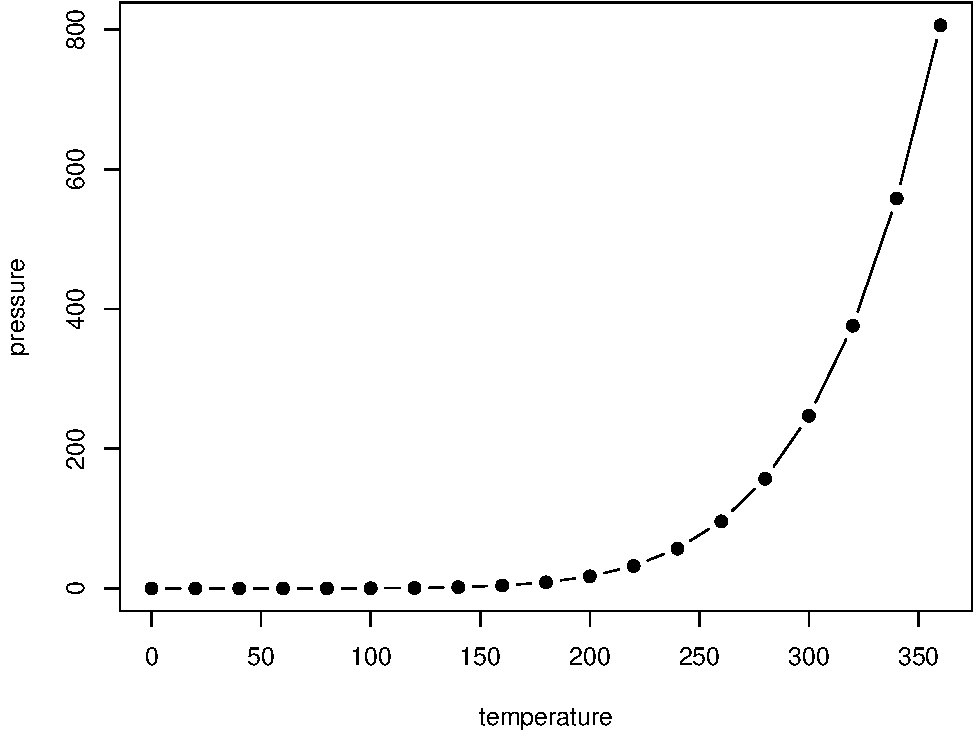
\includegraphics[width=0.8\linewidth]{Defense_files/figure-latex/nice-fig-1} 

}

\caption{Here is a nice figure!}\label{fig:nice-fig}
\end{figure}

Reference a figure by its code chunk label with the \texttt{fig:}
prefix, e.g., see Figure \ref{fig:nice-fig}. Similarly, you can
reference tables generated from \texttt{knitr::kable()}, e.g., see Table
\ref{tab:nice-tab}.

\begin{Shaded}
\begin{Highlighting}[]
\NormalTok{knitr::}\KeywordTok{kable}\NormalTok{(}
  \KeywordTok{head}\NormalTok{(iris, }\DecValTok{20}\NormalTok{), }\DataTypeTok{caption =} \StringTok{'Here is a nice table!'}\NormalTok{,}
  \DataTypeTok{booktabs =} \OtherTok{TRUE}
\NormalTok{)}
\end{Highlighting}
\end{Shaded}

\begin{table}

\caption{\label{tab:nice-tab}Here is a nice table!}
\centering
\begin{tabular}[t]{rrrrl}
\toprule
Sepal.Length & Sepal.Width & Petal.Length & Petal.Width & Species\\
\midrule
5.1 & 3.5 & 1.4 & 0.2 & setosa\\
4.9 & 3.0 & 1.4 & 0.2 & setosa\\
4.7 & 3.2 & 1.3 & 0.2 & setosa\\
4.6 & 3.1 & 1.5 & 0.2 & setosa\\
5.0 & 3.6 & 1.4 & 0.2 & setosa\\
\addlinespace
5.4 & 3.9 & 1.7 & 0.4 & setosa\\
4.6 & 3.4 & 1.4 & 0.3 & setosa\\
5.0 & 3.4 & 1.5 & 0.2 & setosa\\
4.4 & 2.9 & 1.4 & 0.2 & setosa\\
4.9 & 3.1 & 1.5 & 0.1 & setosa\\
\addlinespace
5.4 & 3.7 & 1.5 & 0.2 & setosa\\
4.8 & 3.4 & 1.6 & 0.2 & setosa\\
4.8 & 3.0 & 1.4 & 0.1 & setosa\\
4.3 & 3.0 & 1.1 & 0.1 & setosa\\
5.8 & 4.0 & 1.2 & 0.2 & setosa\\
\addlinespace
5.7 & 4.4 & 1.5 & 0.4 & setosa\\
5.4 & 3.9 & 1.3 & 0.4 & setosa\\
5.1 & 3.5 & 1.4 & 0.3 & setosa\\
5.7 & 3.8 & 1.7 & 0.3 & setosa\\
5.1 & 3.8 & 1.5 & 0.3 & setosa\\
\bottomrule
\end{tabular}
\end{table}

You can write citations, too. For example, we are using the
\textbf{bookdown} package \citep{R-bookdown} in this sample book, which
was built on top of R Markdown and \textbf{knitr} \citep{xie2015}.

\chapter{High Dimensional eQTL}\label{high-dimensional-eqtl}

\section{Motivation}\label{motivation}

Since activation or inhibition of gene expression causes change in
phenotypic formation, the identification of expression quantitative
trait loci (eQTLs) that regulate the pattern of gene expression is
essential for constructing a precise genotype-phenotype map
(\cite{emilsson2008genetics}; \cite{cookson2009mapping};
\cite{nica2013expression}). With the advent and development of various
biotechnologies, it has become possible that genome-scale marker and
expression data can be generated, providing an important fuel to
systematically study the biological function of any types of cellular
components in an organism (\cite{kim2014meta}; \cite{fairfax2014innate};
\cite{lee2014common}). Several genome-wide association studies (GWAS)
have been initiated to map a complete set of eQTLs for the abundance of
genome-wide transcripts whose expression levels are related to
biological or clinical traits
(\cite{nica2013expression};\cite{li2013using};
\cite{koopmann2014genome}). Statistical analysis and modeling are
playing an increasing role in mapping and identifying the underlying
eQTLs from massive amounts of observed data
(\cite{kendziorski2006statistical}; \cite{chun2009expression};
\cite{sun2012statistical}; \cite{flutre2013statistical}).

A typical eQTL mapping approach is to associate a gene transcript with a
single marker such as single nucleotide polymorphism (SNP). By analzying
the significance of all these markers one by one adjusted for multiple
testing, one can count significant loci that contribute to variation of
expression by the gene. This marginal approach based on a simple
regression model has been instrumental for the identifcation of eQTLs in
a variety of organisms (\cite{rockman2010selection};
\cite{kim2014meta}). However, there are two major limitations for the
results by such a marginal analysis: First, it does not take into
account the dependence of different markers, thus a significant
association detected by one marker may be due to the other markers that
are linked with it. The marginal marker analysis cannot separate the
confounding effect of eQTLs due to marker-marker dependence or linkage
(\cite{wu2007statistical}). Second, an eQTL may act through its
interaction with other eQTLs and environmental factors. Because of their
paramount importance in affecting complex diseases and traits, gene-gene
interactions, or epistatic effects, and gene-environment interactions
have been studied intensively in modern biological and medical research
(\cite{cheverud1995epistasis}; \cite{moore2003ubiquitous};
\cite{van2010detection}; \cite{mackay2014epistasis})

These two limitations can be overcome by analyzing all markers and their
pairwise interactions simultaneously through formulating a
high-dimensional regression model. Although it can infer a complete
picture of the genetic architecture of gene expression, this endeavor is
highly challenged by the curse of dimensionality, i.e., the number of
predictors far exceeds the number of observations. The past decade has
witnessed the tremendous development of variable selection models for
high-dimensional data analysis, such as LASSO
(\cite{tibshirani1996regression}), SCAD (\cite{fan2001variable}),
Dantzig selector (\cite{candes2007dantzig}), elastic net
(\cite{zhao2006model}), minimax concave penalty (MCP)
(\cite{zhang2010nearly}) among others. Many methods possess favorable
theoretical properties such as model selection consistency
(\cite{zhao2006model}) and oracle properties (Fan and Lv 2011). When the
number of predictors is much larger than the number of observation, sure
screening is a more realistic goal to achieve than oracle properties or
selection consistency (\cite{fan2008sure}; \cite{wang2009forward}). Sure
screening assures that all important variables are identified with a
probability tending to one, hence achieving effective dimension
reduction without information loss and providing a reasonable starting
point for low-dimensional methods to be applied.

More recently, Hao and Zhang (\cite{hao2014interaction}) extended
variable selection approaches to jointly model main and interaction
effects from high-dimensional data. Based on a greedy forward approach,
their model can identify all possible interaction effects through two
algorithms iFORT and iFORM which have been proved to possess sure
screening property in an ultrahigh-dimensional setting. In this article,
we implement and reform Hao and Zhang's model to map the genetic
architecture of eQTL actions and interactions for gene expression
profiles. This model is modified to accommodate to the feature of a
genetic mapping or GWAS design in which molecular markers as genetic
predictors are discrete although some additional continuous predictors
can also be considered. We expand Hao and Zhang's regression model to
include discrete components. Also, for an F2 or a natural population
with three genotypes at each locus, we need to estimate a total of eight
genetic effects for a pair of markers, which are additive and dominant
effects at each locus, and additive  additive, additive  dominant,
dominant  additive and dominant  dominant effects between the two loci
(\cite{kempthorne1968correlation}). Thus, if the number of markers is p,
a total number of predictors including all main and two-way interaction
terms is \(2p^2\). For a typical moderate-sized mapping study, in which
several thousands of markers are genotyped on a few hundred individuals,
consideration of pair-wise genetic interactions will quickly make the
dimension of predictors an ultrahigh one.

By modeling all markers jointly at one time under an organizing
framework, the modified model can detect all possible significant eQTLs
and their epistasis. An eQTL can be either a cis-QTL, coming from the
same physical location as the gene expression, or a trans-QTL, coming
from other areas of the genome. Our model can more precisely discern
these two different types of eQTLs and their interactions than
traditional marginal analysis. By reanalyzing a published data collected
in a mapping population of C. elegans (\cite{rockman2010selection}), the
new model has validated previous results by the marginal approach,
meanwhile obtained new discoveries on the genetic origin of gene
expression differentiation, which could not be detected in a traditional
way.

Add a paragraph to motivation section Continue on about the rest of the
chapter as an overview

\section{Methods}\label{methods}

\subsection{Experimental design}\label{experimental-design}

Consider an experimental population for genetic studies of complex
traits, such as the backcross and F2 initiated from two inbred lines,
full-sib family derived from two outcrossing parents, or random samples
drawn from a natural population. These types of populations are used
specifically for different species. Although they have different levels
of complexities for statistical modeling, the genetic dissection of
different populations underlies a similar principle. For the purpose of
simplicity, we consider a backcross design in which there are only two
genotypes at each marker.

Suppose the backcross contains n progeny, each of which is genotyped by
p markers, such as single nucleotide polymorphisms (SNPs), distributed
over different chromosomes. The number of SNPs p should be large enough
to completely cover the entire genome at an adequate depth so that we
can possibly capture all possible genetic variants. An increasing body
of evidence suggests that significant SNPs associated with complex
traits or diseases are more likely to be eQTLs (\cite{li2013using}).
Hence the identification of eQTLs is an important first step toward the
genetic dissection of end-point phenotypes. For this reason, we assume
that genome-wide gene transcripts have been available for the assumed
study population. Assume that all progeny are recorded for the same
organ by microarray, leading to expression abundance data of m gene
transcripts. We purport to identify all possible genetic variants
including main effects and interaction effects of SNPs that contribute
to each gene transcript.

\subsection{Adaptation of iFORM
procedure}\label{adaptation-of-iform-procedure}

Hao and Zhang \cite{hao2014interaction} formulated an interaction
forward selecting procedure under the marginality principle (iFORM). The
marker and gene transcript data of the study population can be denoted
as \((X_i,Y_i) (i = 1, …, n)\) which are independent and identically
distributed copies of (X,Y), where X=(X\_1,..,X\_p )\^{}T is a
p-dimensional predictor vector and Y is the response, expressed by a
linear regression model:\\
Y=β\_0+β\_1 X\_1+⋯+β\_p X\_p+ϵ (1) The 's are the coefficients for the
genetic effects of each marker. Like most genome-wide datasets, the
number of markers here grossly outnumbers the number of observations, p
\textgreater{}\textgreater{} n. Therefore, selection procedures would
need to be implemented in order to fit a linear regression model such as
(1). We are already at the point of high-dimensional data but if we want
to include epistatic effects between different markers as predictors as
well it would increase the amount of predictors by (p\^{}2+p)/2 . The
resulting linear model would grow to be, Y=β\_0+β\_1 X\_1+⋯+β\_p
X\_p+γ\_11 X\_1\^{}2+〖〖γ\_12 X〗\emph{1〗}(X\_2 )+⋯+γ\_pp X\_p\^{}2+ϵ
, (2) where 's are the coefficients for the epistatic effects for all
the quadratic and two-way interactions between the markers. For
convenience we will assume that the markers and the transcripts are
standardized before running the selection procedure. Therefore, E(X\_ij
)=0,Var(X\_ij )=1,E(Y\_i )=0 and Var(Y\_i )=1 for i=1,\ldots{},n;
j=1,\ldots{},p. Also, the quadratic and two-way interaction effects will
be centered which we will write as Z\_i=(\ldots{},X\_ik X\_il-E(X\_ik
X\_il ),\ldots{})\^{}T. By doing so we would eliminate the need for an
intercept in regression model (2). This would reduce the model to the
form, \(Y=X^T β+Z^T γ (3)\)

Some notations that will be used to define the elements of
\cite{hao2014interaction} iFORM procedure are as follows.\\
P\_1=\{1,2,\ldots{},p\} P\_2=\{(k,l):1≤k≤l≤p\}. which are the index sets
for the linear and two-way interactions terms, respectively. The
significant main effects for the markers and their interaction effects
are T\_1=\{j:β\_j≠0,j∈P\_1 \},T\_2=\{(j,k):β\_jk≠0,(j,k)∈P\_2 \}. For
any model M, \textbar{}M\textbar{} will be used to denote the number of
predictors contained in the model. The true model size would be
indicated by \textbar{}T\_1 \textbar{}=p\_0 and \textbar{}T\_2
\textbar{}=q\_0 or together would be
\textbar{}T\textbar{}=d\_0=p\_0+q\_0. For the procedure, three sets will
be used throughout. The sets are M for the model set, C for the
candidate set of predictors and S for the solution set of predictors
currently selected in the model.

There are two principles that are used in the selection procedure when
considering interactions as candidates for selection into the final
model. The first is considering the principle of marginality. The
principle states that it is inappropriate to model interaction terms
when the main effects contributing to the interaction have either not
been included in the model or are deleted because their effects become
marginal by the inclusion of the interaction effect. The second
principle important to the procedure is the heredity principle. The
strong case of the principle states that an interaction effect should
not be considered unless both the contributing main effects are in the
model (\cite{zhao2006model}). This would translate to
\(γ_jk≠0 only if β_j 〖,β〗_k≠0 ∀ 1≤j,k≤p\) for model (2). By including
both principles during the selection process it allows for dynamically
including both main effects and interactions effects. The interaction
effects can only be considered between the main effects currently
selected into the solution set of the model according the discussed
principles. A more formal description of the procedure is given below.

\subsection{iFORM}\label{iform}

\cite{hao2014interaction} formulated an interaction forward selecting
procedure under the marginality principle (iFORM). The procedure's
initial step starts with the empty set for both the solution set and the
model set, \(S_0=∅\) and \(M_0=∅\). The candidate set contains all main
effects at the beginning, \(C_0=P_1\), for each of the markers as a
possible eQTL. Typical forward selection procedures are carried out to
start the selection. Each marker is tested individually using a marker
regression. The marker that results in the lowest residual sum of
squares is the marker selected from the candidate set into the solution
set as an eQTL. This is then iterated again for a selection of another
marker into the model set. Once there are at least two main effects
selected into the solution set, using the strong heredity principle, the
quadratic and two-way interactions are then created and placed into the
candidate set as possible eQTLs for selection in the next step. This
process continues selecting main effects or the newly created
interaction effects into the solution set. If another main effect is
selected into the solution set, then the candidate set grows with the
creation of all possible two-way interactions of the main effects that
are currently in the solution set. This is continued until a designated
stopping value, say d. For the number of predictors placed into the
model set from the solution set the Bayesian information Criterion was
used, \(BIC_2 (M ̂ )=loga(σ ̂_M ̂^2 )+n^(-1) |M ̂ |*(loga(n)+2*loga(d^*\) )
), where \(σ ̂_M ̂^2\) is the sample variance for the given model,
\textbar{}M ̂ \textbar{} is the size of the model or the number of
predictors selected into the given model, and n is the sample size. The
\(d^*\) term is the number of predictors in the full model. This was
proposed as \(BIC_2\) by \cite{chen2008extended} which they derived to
help control the false discovery rate in high dimensional data
situations. They also showed that it was selection consistent if
\(d^*=O(n^ξ )\) for some \(ξ>0\). The only difference between the
traditional \(BIC\) calculation and the \(BIC_2\) is the additional term
involving \(2log(d*)\). Ignoring the \(BIC\), the most the number of
steps in the solution path is of size n. The parameter d controls the
overall length of the solution path. In practice, the exact number of
predictors to include, say d\_0, in the true model is unknown. We want
to make d large enough to include d\_0 but not so large as to fit the
model to the point where it becomes oversaturated. Using the \(BIC_2\)
should help avoid such a matter as well. It is reasonable to assume that
d\_0 is much smaller than n in high dimensional sparse regression
problems (\cite{fan2008sure}). Since this is the case, for the purposes
of our model, d was set to be no larger than \(n/loga(n)\). Generally,
the \(BIC_2\) should reach minimum, indicating the optimal stopping
point, before the designated stopping value, is reached.

\subsection{Some considerations}\label{some-considerations}

There were some considerations and pre-processing steps taken before the
iFORM procedure was implemented. The first consideration was to see if
there were any exact duplicate markers in the dataset. One drawback that
could arise with marker datasets when attempting to run multiple linear
regression is the possibility of duplicate markers in the dataset. If
two different markers would happen to have exactly the same genotypes
for each subject it would show up as an exact linear combination of each
other if both markers were to be placed in the linear model. Including
redundant markers in a linear model would not add any additional
information and therefore should not be included in the candidate set
during the selection procedure. This also reduces the dimension slightly
when there are duplicate markers in the dataset.

Another consideration made is the type of coding used for the genotypes.
At any given eQTL, the jth eQTL, say, there are two possible genotypes:
Q\_j Q\_j and Q\_j q\_j, making the total number of possible QTL
genotypes in the population 2\^{}m. The goal of a genetic model is to
relate the 2\^{}m possible genotypic values to a set of genetic
parameters, such that these parameters are interpretable in terms of
main and epistatic effects of the m eQTL. A genetic model is to use
orthogonal contrast scales because it is consistent in the sense that
the effect of a eQTL is consistently defined whether the genetic model
includes one, two, three, or more eQTL (\cite{kao2002modeling}). The
orthogonal contrasts for the genetic model can be expressed by
\(x_ij=■(1/2\) if homozygote \(Q_j Q_j@-1/2\) if heterozygote
\(Q_j q_j\) ) Typically in an inbred line backcross population a given
genotype is coded with a 0 and 1. However there are two draws backs to
this coding when considering the selection procedures discussed above.
The first issue comes with not including an intercept in model (2). If
this is the case each of the predictors would need to be centered making
the coding to -1/2 and 1/2 instead of 0 and 1. Besides meeting the
assumptions of the model that the predictors are centered, it is also
beneficial for the interaction effects as well. If the coding would
remain at 0's and 1's, the interaction coding would also consist of 0's
and 1's. This could propose a problem because three out of the four
scenarios of epistasis between markers would result in a coding of 0 for
the level in the interaction effect. This has the potential to falsely
skew the data of no additive effect for interactions terms because of
the sparseness of coding. By centering the coding to \((-1/2,1/2)\), it
would result in an interaction effect being coded as (-1/4,1/4). This
coding would happen for different scenarios for each of the levels. The
-1/4 could arise when the interaction is made up of a homozygote
interacting with a heterozygote genotype. A coding of 1/4 would arise by
either a homozygote interacting with another homozygote genotype, or
when a heterozygote interacts with another heterozygote genotype.

\section{Application}\label{application}

\subsection{Simulation Results}\label{simulation-results}

Simulations studies were conducted to test the theoretical properties of
the selection procedures and the results \textbf{(Tables 1
-3)\ref{tab:nice-tab}}. The results were compared to several other
commonly used methods for eQTL mapping. In each of the examples the
response was generated from model (2) with σ=1,2,and 3 for the random
error with a sample size of \(n=200\). The \(X_i\)'s were all
independently and identically distributed realizations generated from
\(Binomial(0.5)\) and then orthogonal contrasts were made making each
\(x_ij∈(-1/2,1/2)\). The true \(β=(〖3,0,0,3,0,3,3,0〗_493)\), therefore
making \(T_1={1,4,6,7}\) and \(p_0=4\). The relevant interactions were
set to the pairs \(T_2={(1,6),(1,7),(4,7),(4,7)}\) and \(q_0=4\) all
with \(γ_jk=3\) where \((j,k)∈T_2\). There were several methods compared
during each of the simulations \textbf{(Tables 1 -3)\ref{tab:nice-tab}}.
The methods that were used to model the data were single marker
analysis, forward selection involving only main effects (FS), forward
selection involving all main effects and interaction (FS2) and the iFORM
procedure. Several outcomes were evaluated to compare across each of the
models. The outcomes are separated into three parts. The first part
focuses on the selection of main effects, the second part focuses on the
selection of interaction effects and the third part is the overall model
performance. Simulations of M=100 replicates were run and the outcomes
considered include \emph{Convergence Probability (Cov)
\(∑_(m=1)^M▒〖I(T⊂T ̂ )/M〗\) }Percentage of correct zeros (Cor0)
\(∑_(m=1)^M▒∑_(j=1)^p▒〖I((β_j ) ̂=0,β_j=0)/[M(p-p_0)]〗\)
\emph{Percentage of incorrect zeros (Inc0)
\(∑_(m=1)^M▒∑_(j=1)^p▒〖I((β_j ) ̂=0,β_j≠0)/[M(p_0)]〗\) }Exact Selection
probability (Exact) \(∑_(m=1)^M▒〖I(T=T ̂ )/M 〗\) \emph{The average
model size }Mean Square Error (MSE) \emph{Adjusted R-square }Computation
Time in seconds

In each instance of the simulation, the iFORM procedure was closest to
the simulated data, indicated as Oracle. Single marker analysis was
conducted on each of the main effects individually and the significant
markers were then designated as eQTLs. When comparing the single marker
analysis, we can see it rarely designated the full set of main effects
as significant from the simulated data. Also, no consideration for
interactions could be assessed in single marker analysis. The iFORM
procedure contains the identified main effects over 90\% of the time
across all simulations. The procedure also includes interaction
selection. The interaction screening shares a similar success rate where
the interaction effects are correctly selected over 90\% of the time as
well. Focusing on the computation time, we observed only a few seconds,
on average, increase than running single marker analysis. The final
models selected by the iFORM procedure had similar adjusted R-square
values as the Oracle results, on average. Looking at the exact selection
percentage, we can see that the vast majority of the time the correct
predictors were selected and indicated as significant each time. To
compare the interaction screening effectiveness, forward selection was
implemented on both the main effects and interactions effects. The time
it took to create the design matrix in order to implement forward
selection was not included in the computation time. As can be seen from
the results, using forward selection on the full set of main effects and
pair-wise interactions took substantially longer to run on average than
any of the other methods, including the iFrom procedure. Another
drawback to implementing forward selection on such a large set seemed to
come with over fitting the model. The selection included the maximum
number of predictors allowed by the designated stopping value and did
not use the BIC criteria for final model selection. This resulted in 19
additional predictors selected \textbf{(Tables 1 -3)\ref{tab:nice-tab}}.
This increased the adjusted R-square value of the final model, however
this is suspected because of over fitting the data and not to be a true
prediction of the response.

\subsection{Real Data Analysis}\label{real-data-analysis}

\cite{rockman2010selection} reported an eQTL mapping study of C. elegans
using 208 recombinant inbred advanced intercross lines (RIAIL) from a
cross between the laboratory strain, N2, and a wild isolate from Hawaii,
CB4856. Abundances of 20,000 gene transcripts were measured by
microarray in developmentally synchronized young adult hermaphrodites of
these lines, providing a genome-wide coverage of C. elegans from
WormBase, a public C. elegans genome database. The microarray data was
preprocessed through a normal--exponential convolution background
correction and normalized using quantile standardization. Although they
are closely related, the two strains used for the cross are considered
relatively divergent for C. elegans. The two strains differ roughly at
approximately 1 base pair per 900. Their RIAILs were genotyped at 1454
ordered single-nucleotide polymorphism (SNP) markers that cover the
whole genome of C. elegans including five autosomes (denoted as I -- V)
and one sex chromosome (denoted as X).

\cite{rockman2010selection} used a classic interval mapping approach to
detect 2309 eQTLs by testing and scanning associations of each SNP with
each gene transcript over the entire genome. Rockman et al.'s analysis
allowed a rectangular map of eQTL positions  gene positions to be
constructed (Fig. 1), from which one can identify cis-eQTLs on the
diagonal and trans-eQTLs off the diagonal. However, because their
association analysis was conducted individually for each SNP, the
detection of eQTLs was based on the marginal effects of individual
eQTLs, which may lead to two issues being unsolved. First, of those
eQTLs detected for the same gene transcript, some may include confounded
effects by others. Second, the effects of genetic epistasis may take
place but were not detected. By analyzing all SNPs simultaneously under
a single framework, the high-dimensional model, iFORM, implemented in
this study can more precisely characterize the genetic machineries
underlying variation in each gene transcript. More specifically, we
treat each transcript as a response with all SNP markers and their
interactions as predictors by building a big regression model.
Significant predictors were then selected based on the iFORM procedure.
A final model including both main and interaction effects can be
evaluated by calculating adjusted R-square values

Figure 2 illustrates the map of how a particular gene transcript is
controlled by its eQTLs through main effects and interaction effects.
For clarity of our presentation, we only chose one representative gene
transcript from each chromosome. For example, gene transcript
A\_12\_P103290 located at position 2069088 -- 2069147 of chromosome I
was detected to be controlled by main effects due to X2\_13516256 eQTLs
on chromosomes II and X4\_15632637 eQTLs on chromosome IV and
X2\_13516256:X4\_15632637 interactions between some of these eQTLs on
these two chromosomes.

iFORM provides the estimates of each effect (either main effect or
interaction effect), standard errors of each estimate and the
significance tests of each effect. As an example, Table 4 gives the
result of how gene transcript A\_12\_P103290 can be predicted by its
eQTLs and their interactions. It can be seen that the final predictive
model (adjusted R2 = 0.896) contains 14 markers which exert their main
effects and/or interaction effects on the transcript. Of the 14 final
markers, a half shows significant main effects (p \textless{} 0.05),
with several (i.e., X\_14636404, X4\_15568674, X4\_15632637 and
X\_14542103) explaining about 5\% heritability (defined as a proportion
of genetic variance due to a predictor over the total phenotypic
variance). Of these final markers, we identified eight significant
epistatic interactions. Each epistasis accounts for 4.6 -- 5.5\%
heritability (Table 4).

It is interesting to note that all predictors jointly contribute to
62.6\% heritability for transcript A\_12\_P103290, of which main effects
account for 26.7\% and epistatic effects account for 35.9\%. It is very
surprising that epistasis contributes to more than a half of
heritability. Of the eight epistatic interactions, only one occurs due
to the interaction between two significant eQTLs, X\_14542103 and
X4\_13532205 (Table 4). All the remaining is due to interactions between
one significant eQTL and one non-significant marker. Some eQTLs, such as
X\_14542103 and X\_14636404, produce epistasis with a greater frequency
than others. Despite their involvement in the final predictive model,
some markers were tested to be insignificant in terms of both main and
interaction effects, suggesting that they regulate a gene transcript in
a subtle but important fashion. In summary, iFORM can not only provide
an estimate of the overall heritability of gene transcript
A\_12\_P103290 (i.e., the sum of individual heritabilities explained by
each predictor), but also chart a detailed picture of how each genetic
variant contributes to transcript variation. In particular, iFORM can
characterize epistasis and its role in trait control, thus equipped with
a capacity to retrieve so-called missing heritabilities
(\cite{manolio2009finding}), a significant issue arising from current
genome-wide association studies.

Through analyzing associations between all markers and each transcript
by iFORM, we can identify the difference of cis- and trans-eQTLs for a
particular transcript. For example, of the eQTLs affecting
A\_12\_P103290, we detected that X1\_2068168 is a cis-eQTL, whereas all
others are trans-eQTLs (Table 4). We list the number and distribution of
these two types of eQTLs and the pattern of how they interact with each
other to determine gene transcripts (Table 5). By detecting cis-eQTLs
and trans-eQTLs, iFORM detected that genetic interactions take place
mostly between trans-eQTLs.

\section{Discussion}\label{discussion}

With the recent development of genotyping and sequencing techniques, the
collection of genome-wide genetic and genomic data from any tissue of an
organism has been made much easier and more efficient. Because of this,
genetic studies of complex diseases or traits have developed during the
past decade to a point at which we can draw a complete picture of
genetic architecture for disease or trait formation and progression by
genome-wide association studies (GWAS) (Mackay et al. 2009). Traditional
marginal analysis based on simple regression has been instrumental for
the detection of important genetic variants or quantitative trait loci
in a variety of organisms, but its bottleneck has emerged quickly due to
its limitation in precisely and comprehensively charting genetic control
landscapes. Many GWAS studies published are bothered by missing
heritabilities because of their incapacity to detect genome-wide
epistasis and genotype  environment interactions
(\cite{manolio2009finding}).

Epistasis is a phenomenon by which the influence of a gene on the
phenotype depends critically upon the context provided by other genes
(\cite{cheverud1995epistasis}). It has been increasingly recognized that
epistasis is an important source for trait variation
(\cite{moore2003ubiquitous}; \cite{carlborg2004epistasis};
\cite{cordell2009detecting}), thus inclusion of epistasis would enhance
the prediction accuracy of phenotypic performance and shed more light on
the global genetic architecture of trait control (Mackay 2014). However,
epistasis is extremely hard to detect as an interaction term, whose
inclusion may complicate the inference of the predictive model
(\cite{carlborg2004epistasis}; \cite{mackay2014epistasis}). Thanks to
recent progresses in high-dimensional data modeling, we have been able
to implement several cutting-edge statistical models for systematical
detection and characterization of genome-wide epistasis.

\cite{hao2014interaction} proposed a new high-dimensional model, iFORM,
that can tackle an issue of interaction selection simultaneously from a
large pool of continuous predictors. This model is based on
forward-selection-based procedures, characteristic of computational
feasibility and efficiency. The authors further proved that the
detection of interactions by iFORM is consistent, even if the dimension
increases exponentially for a sample size. As one of the first attempts
to introduce high-dimensional models into genetic studies, we modified
iFORM to accommodate to the discrete nature of molecular markers. Our
simulation studies indicate that iFORM can provide reasonably accurate
and precise estimates of genetic main effect and interaction effects.
Also, it shows greater power to detect significant genes and their
interactions which may not be detected by traditional single marker
analysis.

We applied iFORM to re-analyze gene expression data in an eQTL mapping
study (\cite{rockman2010selection}). While our results confirmed those
by the traditional approach, the new model provides some new findings
including new eQTLs and epistasis, thus allowing a complete set of
genetic variants to be characterized. As an important tool to understand
the genetic mechanisms underlying both complex traits and diseases, eQTL
mapping has been widely used to identify key regulatory pathways toward
endophenotype and end-point phenotypes (\cite{schadt2005integrative};
\cite{emilsson2008genetics}; \cite{cookson2009mapping};
\cite{pickrell2010understanding}; \cite{nica2013expression}). A typical
eQTL study may not only include a large number of molecular markers as
like in a GWAS, but also record tens of thousands of gene transcripts
throughout the entire genome. Our current version of iFORM can only take
into account one gene transcript as a response at a time, thus having a
limitation to model the correlation and dependence among different
genes. It is our next step to formulate a multivariate multiple
regression model by which to test how an individual predictor, main
effect or epistatic effect, pleiotropically affects correlated
expression profiles of different genes.

Given the complexity of biological phenomena, pair-wise epistasis may be
insufficient to explain phenotypic variation.
\cite{imielinski2008exploiting} argued that high-order interactions
among more than two genes may provide a key pathway toward complex
traits. Three-way interactions have been detected in trait control
(\cite{mcmullen1998quantitative}; \cite{stich2007power}). A model for
modeling three-way interactions has been developed in a case-control
GWAS design (\cite{wang2010general}) and a genetic mapping setting
(\cite{pang2013statistical}). It is crucial to extend iFORM to map main
effect, two-way epistasis and three-way epistasis in an eQTL mapping
study although no substantial change is needed in the computational
algorithm, except for an enlarged test set and extra computing time. Our
work is based on a backcross population in which there are only two
genotypes at a locus. The backcross population can facilitate our
estimation and test of genetic effects owing to a smaller number of
parameters at each locus or locus pair, but its utility is very limited
in the F2 design of model systems and natural populations of outcrossing
species such as humans. A more general model of iFORM should consider
three genotypes at each locus, which provides estimates of additive and
dominant effects at each locus and four types of epistasis, i.e.,
additive  additive, additive  dominant, dominant  additive and
dominant  dominant, between each pair of loci
(\cite{kempthorne1968correlation}). Each of these epistatic types may
affect a phenotype through a different pathway.

With continuous falling of sequencing price, we will have desirable
opportunities to study the dynamic behavior and pattern of gene
expression profiles across time and space scales
(\cite{vinuela2010genome}; \cite{ackermann2013impact}). Many previous
studies suggest that gene expression during cell and organ development
may follow a particular form, which can be quantified by mathematical
equations (\cite{kim2010wavelet}). For example, abundance of gene
expression may change periodically in human's brain during circadian
clock. Many researchers used Fourier's series approximation to model the
periodic changes of gene expression by estimating the period and
amplitude of the cycles (\cite{li2013using}). By integrating Fourier
series into iFORM, we will be able to map dynamic eQTLs for gene
expression and make a quantitative prediction of temporal and spatial
patterns of genetic control by eQTLs.

\chapter{High-order Epistatic
Networks}\label{high-order-epistatic-networks}

\section{Motivation}\label{motivation-1}

\textbf{Shoot-Root Manuscript} Following Sun et al.'s
\cite{sun2014model} developmental model, we calculated and chose four
key heterochronic parameters, asymptotic growth (a), relative growth
rate (r), the timing of inflection point (TI), and the duration of
linear growth (L), as phenotypic values to perform QTL mapping. A great
variability was observed for growth curve parameters of both phenotypic
traits (Table 1). Compared with taproot length, shoot length has a
greater rate of growth and reaches the maximum growth rate at an earlier

\textbf{Start of My Paper} Quantitative traits are very difficult to
study because these traits are controlled by many genes that interact in
a complicated way (Nelson et al. 2013; Mackay 2014). Genome-wide mapping
and association studies increasingly available due to next-generation
high-throughput genotyping techniques have proven to be useful for
characterizing gene-gene interactions, coined epistasis, that contribute
to phenotypic variation (Cordell 2009; Van Steen 2012; Wei et al. 2014).
Powerful statistical methods have been developed to analyze all possible
markers simultaneously, from which to search for a complete set of
epistasis for quantitative traits (Li et al. 2015: Gosik et al. 2016).
The joint analysis of all markers is particularly needed to chart an
overall picture of genetic interactions, in comparison with
computationally less expensive marginal analysis.

Epistasis reported in the current literature is mostly due to
interactions between two genes. However, a growing body of evidence
shows that genetic interactions involving more than two loci play a
pivotal role in regulating the genetic variation of traits (Wang et al.
2010; Dowell et al. 2010; Pang et al. 2013; Taylor and Ehrenreich 2015).
For example, in a mapping population deriving from crossing two chicken
lines, three-locus interactions were detected to determine body weight
(Pettersson et al. 2011). A mapping study established by two yeast
strains identified genetic interactions involving five or more loci for
colony morphology (Taylor and Ehrenreich 2014). Other studies have
demonstrated that high-order epistasis is of critical importance in
regulating metabolic networks in yeast (Weinreich et al. 2013) and
Escherichia coli and Saccharomyces cerevisiae (Imielinski and Belta
2008; He et al. 2010), whereas lower-order (pairwise) epistasis may be
insufficient to explain metabolic variation for these organisms.

The theoretical models of high-order epistasis have well been
established by mathematical biologists (Hansen and Wagner 2001;
Beerenwinkel et al. 2007). These models provided a foundation to
interpret high-order epistasis from a biological standpoint. A few
statistical models have been derived to estimate and test high-order
epistasis in case-control designs (Wang et al. 2010) and
population-based mapping settings (Pang et al. 2013). Wang et al. (2015)
developed a Bayesian version of detecting high-order interactions for
both continuous and discrete phenotypes. However, these models were
based on a marginal analysis, thus less powerful to illustrate a global
view of genetic control mechanisms due to high-order epistasis.

In this article, we deploy a variable selection procedure within a
genetic mapping or association setting to characterize the genetic
architecture of complex traits composed of main effects of individual
genes, pairwise epistasis between two genes, and three-way epistasis
among three genes. The model was built on greedy interaction screening
forward selection developed under the marginality principle (named
iFORM) by Hao and Zhang (2014). These approaches, proved to possess sure
screening property for ultrahigh-dimensional modeling, have been
implemented to model the genetic architecture of main effects and
pairwise epistasis due to eQTLs for gene transcripts (Gosik et al.
2016). Here, we extend the implementation of iFORM to systematically
capture three-way interactions that are expressed among all possible
markers studied. To show the statistical power of the extended model, we
performed computer simulation studies. The model was further validated
through analyzing a real data of genetic mapping for shoot growth in a
woody plant, mei (Prunus mume). The model should be used in any other
mapping or association studies of quantitative traits.

Add a paragraph to motivation section Continue on about the rest of the
chapter as an overview

\section{Methods}\label{methods-1}

\subsection{Mapping and association
studies}\label{mapping-and-association-studies}

Genetic mapping and association studies are two types of designs used to
dissect quantitative traits. The former is based on a controlled cross
derived from distinct parents, whereas the latter samples different
genotypes from a pool of accessions or a natural population. In both
types of design, a set of individuals are sampled to be phenotyped for
quantitative traits of interest and genotyped by molecular markers
distributed throughout the entire genome. For a particular genetic
experiment, the number of markers is much larger than that of samples,
thus, it is impossible to estimate the genetic effects of all markers
simultaneously using traditional regression models. This issue becomes
much intractable when we aim to estimate genetic interactions of
different orders. To tackle the issue of the number of predictors
\textgreater{}\textgreater{} the number of samples, several variable
selection approaches have been implemented in association studies. One
approach is forward selection which was shown to be robust for
estimating pairwise interactions of predictors (Hao and Zhang 2014).
With sure screening properties and controlling for false positives, this
approach, named iFORM, performs very well in capturing important
information in explaining the response variable. On top of these nice
theoretical properties it is computationally efficient by using ordinary
least squares calculations and only requiring a predetermined set up
steps. Here, we extended the iForm procedure to include HGI's to capture
more relevant information. In the following sections, the notation and
model set-up will be introduced. After this theoretical properties will
be explored. Finally simulated and real data analysis will be conducted
to help confirm the theoretical properties and show the feasibility of
using the model for screening across whole genomes to more precisely
explain phenotypes of interest.

\subsection{Epistatic model}\label{epistatic-model}

Consider a linear model that underlies the true genotype-phenotype
relationship. Assume that the phenotype, as the response of the model,
is controlled by a set of p SNPs that act singly and/or interact with
each other. These main and interaction effects of markers, i.e., the
predictors of the model, need to be estimated. Let Y = (y1, \ldots{},
yn)T denote the phenotypic value of n samples from a mapping or
association population. When considering pairwise and three-way
interactions, the linear model is expressed as Y=〖α+X〗\^{}T β+Z\^{}T
γ+W\^{}T η+ϵ (1) where X=(X\_1,\ldots{},X\_p )\^{}T is the design matrix
that specifies the genetic effects of each marker  = (1, \ldots{}, p)
, Z=(X\_j X\_k )\^{}T (1≤j≤k≤p) is the design matrix that specifies the
epistatic effects between two markers, expressed in γ, W=(X\_j X\_k X\_l
)\^{}T (1≤j≤k≤l≤p) is the design matrix that specifies the epistatic
effects among three markers, expressed in η, and
ϵ\textasciitilde{}N(0,σ\^{}2 ) is the residual error normally
distributed with mean zero and variance σ\^{}2. We denote the index sets
for the linear, order-2 and order-3 effects in equation (1),
respectively, as P\_1=\{1,2,\ldots{},p\}\\
P\_2=\{(j,k):1≤j≤k≤p\} P\_3=\{(j,k,l):1≤j≤k≤l≤p\} With the significant
main, order-2 interaction and order-3 interaction effect sets being,
T\_1=\{j:β\_j≠0,j∈P\_1 \} T\_2=\{(j,k):γ\_jk≠0,(j,k)∈P\_2 \}
T\_3=\{(j,k,l):η\_jkl≠0,(j,k,l)∈P\_3 \}

The true size of T\_1, will be p\_1 and similarly for T\_2 and T\_3 will
have sizes p\_2 and p\_3 respectively. There will be a total of 3 sets
referred to throughout the procedure, the candidate set C, the selection
set S and the model set, M. The candidate set is the set of all possible
predictors at a given step in the selection process. The selection set
contains the predictors that have previously been selected from the
candidate set from each iteration of the procedure. Finally, the model
set is the final model that is fit from the selection set at the end of
the procedure. The BIC is used to determine the optimal cutoff for the
final model size.

\subsection{iForm with high-order
epistasis}\label{iform-with-high-order-epistasis}

The iForm procedure is a forward selecting procedure. In traditional
forward selection the procedure starts with the empty set and then
iterates through the entire set of possible predictors in C and selects
the best predictor and includes it in S at the end of each step. The
best predictor can be determined in many ways but usually is defined by
the predictor that results in the least amount of error. For our
purposes we use the residual sum of squares. This continues with
selecting the best predictor from C at each step until a designated
stopping criterion is met or until some information criterion is met.
Common information criteria used for selecting predictors to be in M are
AIC, BIC, R\^{}2 and Mallow's C\_p statistic.

The iForm procedure for high-order epistatic detection parallels the
forward selection procedure, but C will grow dynamically with the
creation of order-2 and order-3 interaction effects between main effects
that were included from previous iterations of the procedure. There are
three steps to the model selection. The first step is to initialize the
3 sets mentioned above. The sets, S and M are set to the empty set while
the candidate set, C, is first set to P\_1, all the main effects. The
next step starts the forward selection procedure selecting predictors
from C. The selected predictor will be a main effect at the first step.
At subsequent steps, after interaction effects are included, selected
predictors could be either be a main effect, order-two or order-three
interaction effect. The final step involves repeating the second step
until a designated stopping criterion is met. This can be a certain
amount of predictors to be considered in the final model, or it can be
based off of other factors such as the sample size. The designated
stopping criterion will be denoted as d. For our purposes we use d as a
function of the sample size, d = n/lo g\_2a(n). The procedure will run
up until d iterations, and the optimal model will then be constructed
from the selection set. This is done by an information criterion. Here
we used the Bayesian Information Criterion proposed by Chen and Chen
(2008) denoted as the BIC\_2. This was derived by them to control the
false discovery rate in high dimensional model selections.

BIC\_2 (M ̂ )=loga(σ ̂\_M ̂\^{}2 )+n\^{}(-1) \textbar{}M ̂
\textbar{}\emph{(loga(n)+2}loga(d\^{}* ) ) (2)

Once the selection procedure is done and there are d predictors in the
selection set the BIC is used to determine the cutoff value for the
optimum number of predictors in the model set. Then linear regression is
performed on the model set.

Two guiding principles are used to help dynamically select the main
effects and epistasis effects throughout the procedure. The first is the
marginality principle, which states that an effect will not be removed
from the model once it has been selected. A previous selected effect may
become marginal by the inclusion of subsequent effects. This especially
can be the case when an interaction effect is included. One of the
parent effects may become less significant or even not significant at
all by considering both in the model. The next principle we state as the
heredity principle but has also been referred to in other work as the
hierarchy principle (Bien et al 2013 and Lim and Hastie 2014).

The heredity (hierarchy) principle help reduce the search space by
making the assumption that previously selected main effects would be
involved in the interaction effects. By considering this principle it
substantially reduces the search space making this feasible for
ultra-high dimensional situations. Even larger than ram datasets can be
used with efficient memory mapping of the dataset while running the
procedure. The weak version of the heredity principle for three-way
interactions states that at least one of the main effects needs to be
selected into the model to consider an interaction effect that contains
that predictor. Considering a moderately high set of predictors say p =
5000, if trying to include all order-2 interactions upfront, will make
the candidate set be as high as 12,498,000. This alone could exceed most
ram requirements of standard computers. This is before even stepping up
to order-3 interactions. The weak heredity principle would decrease the
candidate set substantially. Assuming a sample size of n = 200, would
give a cut off of n/ lo g\_2a(n) =200/lo g\_2a〖(200)〗 =26 steps in the
procedure. This would give a maximum of approximately 135,000 candidate
predictors. This gives a 100 fold decrease in the candidate set. This
could substantially make ultra-high dimensional analysis more feasible
and also speed it up in the process. This is the weak case. If
considering the strong case the decrease in candidate space is even more
apparent. Aside from the efficiency by lowering the search space of the
candidate set, the heredity principle is usually taken into account by
researchers when selecting models involving the consideration for
interaction effects.

\subsection{Theoretical Properties}\label{theoretical-properties}

The theoretical properties of the iForm procedure with high-order
epistasis follow closely with the forward selection procedure. Hao and
Zhang (2014) summarize forward selection nicely as follows. At each
step, the response is regressed on the most correlated covariate, and
the residual is calculated and used as the new response in next step.
After the most correlated covariate (say, X1) is selected, all other
covariates are regressed on X1, and then the covariates are substituted
by the corresponding normalized residuals, which are used as the new
covariates in next step. By viewing forward selection in this sense the
computational complexity of the procedure depends upon the size of the
candidate set. The candidate set in the iForm's case does grow
dynamically at each step, by at most the number of predictors currently
selected in C for each step. If we denote the current size of the
candidate set as m then each iteration of the procedure grows with
complexity of O(nm), where n is the sample size. Leaving the selection
unrestricted we would not be able to fit more than n predictors for a
linear model and therefore n would be the most main effects that would
be able to be selected. Considering the weakest form of the heredity
principle at the current iteration there would be at most
p+(n(n-1)(n-2))/6 predictors in the candidate set. This would make the
total complexity of the selection procedure to be
nO(n(p+n(n-1)(n-2)))=O(n\^{}3 p+n\^{}5 ). This makes the total
complexity grow linearly as p grows.

The theoretical properties of the iForm procedure show sure screening
properties (Fan et al. 2007). By this we mean that all the import
predictors, whether that is a main effect or epistatic effect will be
selected with probability tending to 1. This is important to capture as
much of the signal as possible through all the noise that comes with p
\textgreater{}\textgreater{} n or ultra-high dimensional situations. It
is also important not to `over-fit' the model with unnecessary
predictors that actually explain more noise in the data that the model
is being fitted on than the actual signal you would like to pick up on.

To show the property from above the following conditions would need to
be met for regulatory purposes. Hao and Zhang (2014) showed how under
these conditions sure screening properties for interaction models like
FS2 and iForm are satisfied. This also applies to order-3 interaction
models like FS3 and iForm with higher order epistasis, like we do with
the high-order epistasis model. The following assumptions need to be met
for these conditions. The first is that the X=(X\_1,\ldots{},X\_p )\^{}T
are jointly and marginally normal with independent normally distributed
error. Next we would need the eigenvalues of the covariance matrix to be
positive and bounded by two constants 0

\chapter{iForm Functional Mapping (A computational
method)}\label{iform-functional-mapping-a-computational-method}

\section{Motivation}\label{motivation-2}

\textbf{Shoot-Root Paper} (The genetic architecture of shoot-root
covariation during seedling emergence of a dessert tree, Populus
euphratica)

Since most traits associated with growth and development can be better
described by a dynamic process (\cite{hernandez2015understanding},
\cite{muraya2017genetic}), it is more biologically meaningful to map
these traits as growth curves (Sun and Wu, 2015). Several approaches
have integrated growth equations into the likelihood of genetic mapping,
leading to the birth of a so-called functional mapping model (Ma et al.,
2002; Wu and Lin, 2006; Li and Sillanpaa, 2015; Muraya et al., 2016).
Functional mapping allows the developmental change of genetic control to
be characterized across time and space (He et al., 2010; Li and Wu,
2010). By modeling the longitudinal mean-covariance structures using a
set of parsimonious parameters, functional mapping has proven of great
statistical power in gene identification and the utilization of sparse
phenotypic data (Hou et al., 2005, 2006). An alternative to functional
mapping is to map growth QTLs by estimating growth parameters for each
genotype based on growth equations and associating these parameters with
markers (Wu et al., 2002).

From fundamental principles of biophysical and biochemical processes,
logistic equations that capture different stages of organ development
have been derived, which show robust biological relevance (West et al.,
2001). Sun et al. (2014) dissect logistic growth curves into several key
landmarks of development using the concept of heterochrony, defined as
the asymptotic growth, relative growth rate, the timing of inflection
and the duration of linear growth.

\textbf{from research statement}

Treating the molecular biology of an organisim as a complex trait, it
would be likely that the expression profiles of certain genes, proteins
or other metabolites would follow a more functional or dynamic
phenotype. This information could be lost or greatly limited by treating
the response as a single static predictor. In an attempt to capture all
relevant information available I am currently extending the procedure
further to include the entire growth function as a phenotype. The mean
growth curve is estimated for the sample and then orthogonal polynomials
are used to assist in fitting the genetic effects for each marker or
interaction between the markers. This would allow the genetic effect
some flexibility over time and give a more representative fit. I
anticipate submitting a third manuscript in late spring around this
topic. This could also be used with other semi parametric functions to
model dynamics or other types of non-linear functions that characterizes
the biological systems being evaluated.

\subsection{Update}\label{update}

(This is from Han Hao's proposal, update for yours)

Changes in developmental timing and rate, named as heterochrony, have
long been believed to be a major force in the evolution of phenotype
(Gould, 1977; Wilson et al., 1988). It has been observed that relatively
few genetic changes in heterochrony through the endocrine regulation of
metamorphosis can cause profound morphological consequences (Moss,
2007). For example, although humans and chimpanzees are closely related,
their skull shape and brain growth are different dramatically during
early development (Rice, 2002; Mitteroecker et al., 2004; King, 2004). A
recent phylogenic investigation revealed that changes in developmental
timing are a crucial step for birds to evolve from dinosaurs (Bhullar,
2012). The consequence of these changes leads birds to take months to
reach sexual maturity, allowing them to retain the physical
characteristics of baby stages characterized by dinosaurs that take
years to mature. One question that naturally arises from these
evolutionary divergences is what mechanisms are implicated for
heterochrony and the change of biological clock.

Many studies have pursued to identify the molecular control of
developmental timing; mostly using Caenorhabditis elegans as an example,
these studies have identified heterochronic genes that orchestrate the
timing of cell divisions and fates during development regulated by
microRNAs and their targets (Ambros, 2000; Rougvie, 2001; Pasquinelli
and Ruvkun, 2002; Banerjee and Slack, 2002; Moss, 2007). Focusing on
particular pathways causing heterochonic changes, none of these studies
has provided an entire picture of the genetic control of heterochrnoy.
Furthermore, the effects of heterochronic genes on the evolution of
complex phenotypes have not been quantified, limiting the inference and
prediction of evolutionary changes.

In this chapter, we develop a general framework for characterizing the
genetic architecture of heterochrony based on widely used genetic
mapping approaches. Genetic mapping has been proved to be powerful for
mapping and studying quantitative trait loci (QTLs) involved in complex
traits (Lander and Botstein, 1986), and has been increasingly integrated
with network biology to better elucidate the mechanisms of the way QTL
acts and interacts with other factors (Wang et al., 2012b). In the
decade, genetic mapping has developed to a point at which this approach
can characterize QTLs that control the process of development, leading
to the birth of functional mapping (Ma et al., 2002; Wu and Lin, 2006;
Li and Wu, 2010). Functional mapping implements mathematical aspects of
developmental principles into a mapping framework, equipped with a
capacity to study the interplay between QTLs and development. Here, we
extend functional mapping to characterize QTLs controlling heterochrony
(named hQTLs), specified by three parameters (i) the onset of a
particular process, (ii) its offset, and (iii) the rate at which the
process proceeds. By using growth equation as an example, we exemplify
the procedure of model derivations as well as the practical use of the
model in hQTL detection. In the end, we discuss an issue of how hQTLs
can be integrated with developmental evolutionary biology (evo-devo), a
fast-growing discipline of biology in the recent years.

Add a third paragraph to motivation section Continue on about the rest
of the chapter as an overview

\section{Methods}\label{methods-2}

\subsection{Functional Mapping}\label{functional-mapping}

\textbf{Update} (This is from Han Hao's proposal, update for yours)

Functional mapping is a group of methods used for mapping QTLs related
to functional valued traits that are measured over a certain time
period. These function-valued traits are widely seen in growth analysis,
shape analysis, network analysis, and clinical trials. By integrating
functional features with genetic analysis, functional mapping methods
often help to increase the statistical power and the biological
relevance between the detected QTLs and biological traits. Functional
mapping methods were first developed using parametric curves to describe
the functional valued traits, such as growth curves or pharmacodynamic
models (Ma et al., 2002; Lin et al., 2005). Later, semi-parametric and
non-parametric models were introduced for complex traits that do not
have specific mathematical forms (Das et al., 2011, 2013).

The key of functional mapping methods is the modelling of both
functional means and the covariance structure across measurements from
the same individual. When modelling the functional means, biological
background is first examined to select the best function, either
parametric or non-parametric. The covariance structure is usually
modeled by parsimonious and flexible approaches such as autoregressive,
antedependence, or nonparametric structures. The functional means and
covariance structures can be integrated into a likelihood function, then
hypothesis testing can be performed with a likelihood ratio testing
approach.

\textbf{Shoot-Root Paper} (pages 13 - 14) fitted by a three-parameter
growth equation, through a nonlinear least-square approach, which is
expressed as (1) where g(t) is the trait value at time t, and three
parameters a, b and r have different biological meanings: a is the limit
value of g when t→∞, r is the relative growth rate, and a/ (1 + b)
denotes the initial value of g when t = 0. After the three growth
parameters were estimated for each progeny, we further determined
heterochronic parameters, i.e., the timing of inflection point (tI), the
timing of maximum acceleration (ta), the timing of maximum deceleration
(td), and the duration of linear growth (L) (Sun et al., 2014).

QTL mapping: For each progeny, we estimated a series of heterochronic
parameters using equation (1) and then treated these estimates as
phenotypic values to perform QTL mapping. There are two statistical
approaches for QTL mapping, mixture model for sparse molecular markers
and multiplicative model for dense markers. Because the linkage map
constructed is quite dense, we employed the multiplicative model that
assumes QTLs are located at the positions of markers. For the same
heterochronic parameter expressed in shoot length and taproot length,
the multiplicative likelihood model is expressed as (2) where  is the
unknown parameters; yi = (y1i, y2i) is the growth parameter vector of
progeny i for shoot length (coded by 1) and taproot length (coded by 2);
nj is the number of progeny with SNP genotype j; and fj(yi) is a
bivariate normal distribution for progeny i with the expected mean
vector for genotype j (1j, 2j) and the variance-covariance matrix 
containing the variances (12, 22) and correlation between the two
traits (). Statistical methods based on the likelihood (2) have been
established to estimate the model parameters  = (1j, 2j, 12, 22,
).

\subsection{Legendre Polynomials}\label{legendre-polynomials}

\subsection{Model}\label{model}

\subsubsection{BIC}\label{bic}

From the book BibTex \citet{book}\{wu2006nonparametric,
title=\{Nonparametric regression methods for longitudinal data analysis:
mixed-effects modeling approaches\}, author=\{Wu, Hulin and Zhang,
Jin-Ting\}, volume=\{515\}, year=\{2006\}, publisher=\{John Wiley \&
Sons\} \}

Similarly, following the classical BIC rule (Swartz 1978), we can define
the BIC rule for the cubic MESS model as

\[BIC(\lambda, \lambda_v ) = -2*LogLik + log(n)*(df + df_v)\] n is the
number of subjects \[\lambda = smoothing paramter\]
\[\lambda_v = smoothing paramter, number of knots in the cubic spline\]

\section{Application}\label{application-1}

\subsection{Simulation Studies}\label{simulation-studies}

\subsection{Worked Example}\label{worked-example}

\chapter{Conclusions}\label{conclusions}

\section{Summary}\label{summary}

\section{Discussion}\label{discussion-1}

Further investigations are needed to confirm or modify our findings by
QTL mapping in natural populations.

\section{Future Steps}\label{future-steps}

\subsection{Aim 1}\label{aim-1}

\subsection{Aim 2}\label{aim-2}

\subsection{Aim 3}\label{aim-3}

We have finished a nice book.

\chapter*{Conclusions}\label{conclusions-1}
\addcontentsline{toc}{chapter}{Conclusions}

\bibliography{packages,book}


\end{document}
